\section{Method}
\label{sec:method}
\subsection{Logistic Regression}
Baseline model

\subsection{Deep Learning Model - CNN}

\begin{figure}[h]
	\centering
	\captionsetup{justification=centering}
	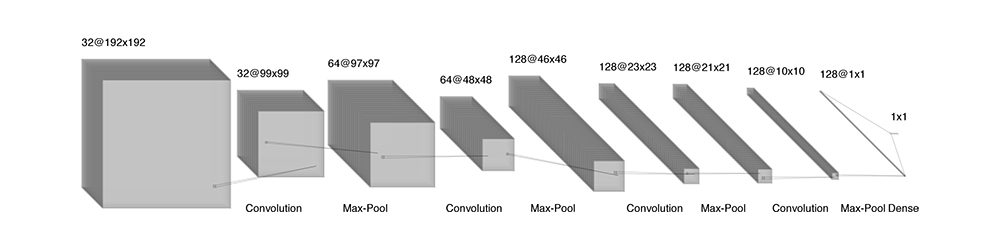
\includegraphics[width=\columnwidth]{Figures/CNNArchitecture.jpg}
	\caption{Architecture of the CNN model}
	\label{fig:cnnarch}
\end{figure}

Deep Learning has achieved significant results and a huge improvement in visual detection and recognition with a lot of categories. Raw data images are used by deep learning as input without the need of expert knowledge for optimization of segmentation parameter or feature design. We used open source software stacks for our project. The deep learning APIs used are Keras and Tensorflow. The proposed architecture of the deep network for the morphological classification is illustrated in detail in Figure~\ref{fig:cnnarch}. It consists of 15 layers, made up of 5 main layers for features extraction, followed by two principle fully connected layers for classification. The first layer is the input layer. Every main layer is further made of one convolutional layer with the Rectified Linear Unit(ReLU) as the nonlinear activation function and a max pooling layer at the end for subsampling. The first fully connected layer has 128 neurons with ReLU activation function, while the last fully connected layer has one neuron and uses a sigmoid to obtain class memberships. Visualizing the feature extraction and classification layers in the proposed deep neural architecture will give a better understating. In the main layers, features are extracted and the patterns identified become more complex as we go deeper into the network. CNNs are generally used for image classification but they are also very useful for finding patterns in any data that can benefit from filters. Using a 5 channel raw input is not typical when employing CNNs but since the image data(RGB) for the galaxy is a subset of the wavelength range of the 5 channels a CNN is very well suited for this classification task. This becomes more apparent with the results(accuracy) of the model.